% !TeX root = main.tex
% !TeX spellcheck = de_DE

\subsection{Fast Fourier Transform}\label{sec:fft}

\begin{definition}[DFT]
    Gegeben eine endliche Folge von Koeffizienten $a:=(a_0,a_1,\ldots,a_{n-1})\in\IC^n$ heißt die Folge $\hat{a}:=(\hat{a}_0,\hat{a}_1,\ldots,\hat{a}_{n-1})\in\IC^n$ der Zahlen gegeben durch
    \[\hat{a}_i := \sum_{j=0}^{n-1} a_i \zeta_n^{-ij}\]
    die \udot{diskrete Fourier-Transformation}\footnote{Jean-Baptiste Joseph Fourier, 1768--1830, franz. Mathematiker und Physiker}, kurz \udot{DFT}, von $a$, wobei $\zeta_n\in\IC$ eine primitive $n$-te Einheitswurzel ist, d.h. $\zeta_n^n=1$ und $\zeta_n^i \neq 1$ für $i<n$, beispielsweise $e^{2\pi i / n}$.

    \medskip
    Das umgekehrte Problem, aus $\hat{a}$ wieder $a$ zu rekonstruieren, heißt entsprechend \udot{inverse DFT}.
\end{definition}

\begin{remark}
    Die DFT ist allgemein für unstrukturierte Folgen von Zahlen definiert, weil sie in vielen verschiedenen Zusammenhängen auftritt, in denen diese Zahlenfolgen unterschiedliche Bedeutung und Herkunft haben.

    Für unser Ziel ist es aber zweckmäßig, die Zahlen $a$ als Koeffizienten eines Polynoms
    \[\alpha(X) := a_0 + a_1 X + \ldots + a_{n-1}X^{n-1} \in\IC[X]\]
    aufzufassen. Dann ist nämlich $\hat{a}_i = \alpha(\zeta_n^{-i})$.
\end{remark}

\begin{lemma}
    Es stellt sich heraus, dass die iDFT im Wesentlichen genauso aussieht wie die DFT selbst. Mit den Bezeichnungen von oben gilt:
    \[a_i = \frac{1}{n}\sum_{k=0}^{n-1} \hat{a}_k \zeta_n^{ik}\]
\end{lemma}
\begin{proof}
    Definitionsgeschubse.
\end{proof}

\begin{remark}
    Eben weil es so viele verschiedene Arten gibt, in denen die DFT auftreten kann, gibt es verschiedene Konventionen, die Definition zu schreiben, die aber im Wesentlichen äquivalent sind.

    So kann man z.B.\ das andere Vorzeichen wählen und stattdessen $\alpha$ in $\zeta_n^{+i}$ auszuwerten. Da $\set{1, \zeta_n, \zeta_n^2, \ldots} = \set{1, \zeta_n^{-1}, \zeta_n^{-2}, \ldots}$ ist, führt das nur dazu, dass die Komponenten von $\hat{a}$ in einer anderen Reihenfolge auftreten, aber ansonsten die gleichen Werte haben.

    Manchmal wird der Faktor $\frac{1}{n}$ auch für die DFT anstelle der iDFT verwendet. Beides zusammen führt im Wesentlichen dazu, dass das, was wir jetzt als iDFT bezeichnen, zur DFT erklärt wird und umgekehrt. Da Hin- und Rückrichtung aber sowieso zum Verwechseln ähnlich ist, macht das auch keinen großen Unterschied mehr, welche von den beiden Operationen man als DFT und welche man als iDFT bezeichnet.

    Manchmal wird der Faktor einfach gleichmäßig verteilt, sodass in beiden Formeln ein $\frac{1}{\sqrt{n}}$ vorkommt.
\end{remark}

\begin{theorem}[Gauss \cite{gauss1866nachlass}, Cooley-Tukey \cite{cooley-tukey} uvm.]
    Ist $n$ eine Zweierpotenz, so ist möglich, die DFT eines Vektors $a\in\IC^n$ mit $n\log(n)$ komplexen Additionen und Multiplikationen und $n+O(1)$ Speicherbedarf zu berechnen.
\end{theorem}

\begin{remark}
    Dieser Algorithmus wurde mehrfach wiederentdeckt. Die zugrundeliegende Idee war bereits Gauss im Jahr 1805 bekannt\footnote{Bevor Joseph Fourier die Fourier-Transformation überhaupt erfunden hatte!}, aber Gauss fand sie nicht wichtig genug, um sie zu veröffentlichen.

    Der Algorithmus wurde im 20.\ Jahrhundert mehrfach wiederentdeckt, u.A.\ von Danielson\&Lanczos in 1942~\cite{danielson_lanczos} und I.Good in 1957~\cite{good}. Dies waren teilweise nur Spezialfälle, teilweise ist die Bedeutung des Ergebnisses nicht als etwas Besonderes erkannt worden. Cooley\&Turkey entdeckten in 1965 unabhängig den allgemeinen Algorithmus und analysierten dessen asymptotische Laufzeit.
\end{remark}

\begin{remark}
    Die Annahme, dass $n$ eine Zweierpotenz ist, ist in der Tat überflüssig. Sie ist nur für den konkreten Algorithmus nötig, den wir jetzt besprechen wollen. Es gibt andere Algorithmen, die für andere $n$ funktionieren und ebenfalls in $O(n\log(n))$ sind.
\end{remark}
\begin{proof}
    Wir werden die DFT als Auswertung des Polynoms $\alpha$ in den $n$ Punkten
    \[\zeta_n^0, \zeta_n^1,\zeta_n^2 \ldots, \zeta_n^{n-1}\]
    betrachten.

    \smallskip
    Die erste nützliche Beobachtung ist, dass wir $\alpha$ hier in Wirklichkeit als Element von $\IC[X]/(X^n-1)$ auffassen können, da die Auswertung in $n$-ten Einheitswurzeln eh keinen Unterschied zwischen $X^n-1$ und $0$ feststellen kann, da ja $\zeta^n-1=0$ ist. Der Ring $\IC[X]/(X^n-1)$ wird nun mittels des chinesischen Restsatzes rekursiv in kleinere Ringe zerlegt:

    Dabei benutzen wir in jedem Schritt, dass $X^{2k}-z^2 = (X^k-z)(X^k+z)$ gilt und das eine Zerlegung in paarweise teilerfremde Faktoren ist (wenn $z\neq 0$), sodass wir den chinesischen Restsatz tatsächlich anwenden können. So erhalten wir in jedem Rekursionsschritt eine Zerlegung in zwei kleinere Ringe jeweils halber Dimension.

    Da $n$ eine Zweierpotenz, $\zeta_n$ eine $n$-te Einheitswurzel und $1=\zeta_n^n$ ist, kann man per Induktion zeigen, dass man in jedem Schritt Faktoren der Form $X^k-\zeta_n^{ak}$ erhält.

    \medskip
    Am Beispiel von $n=8$ sieht das so aus wie in Abbildung~\ref{fig:fft:example_n_equals_8} dargestellt.

    \begin{figure}[htp]
        \centering
        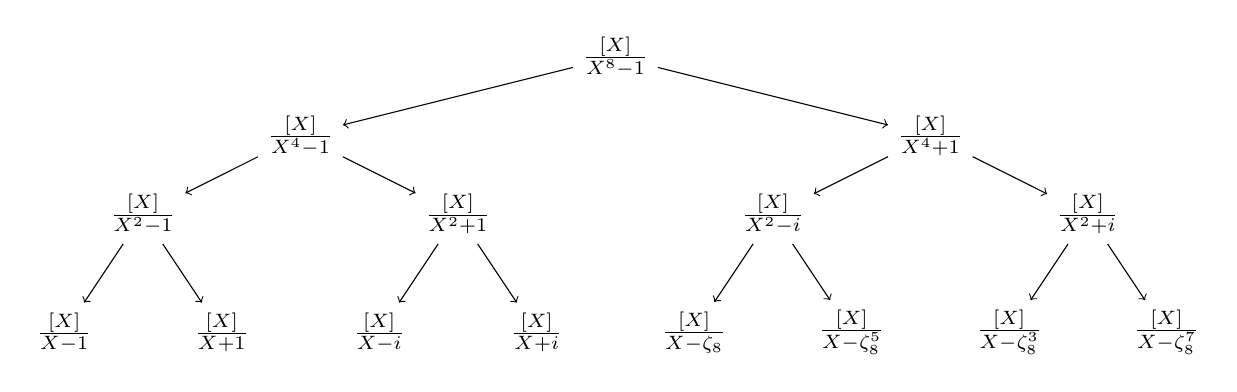
\begin{tikzpicture}
            \node (C8)   at  (0,3) {$\frac{\IC[X]}{X^8-1}$};
            \node (C4-1) at (-4,2) {$\frac{\IC[X]}{X^4-1}$};
            \node (C4+1) at (+4,2) {$\frac{\IC[X]}{X^4+1}$};
            \node (C2-1) at (-6,1) {$\frac{\IC[X]}{X^2-1}$};
            \node (C2+1) at (-2,1) {$\frac{\IC[X]}{X^2+1}$};
            \node (C2-i) at (+2,1) {$\frac{\IC[X]}{X^2-i}$};
            \node (C2+i) at (+6,1) {$\frac{\IC[X]}{X^2+i}$};
            \node (C1-1) at (-7,-0.5) {$\frac{\IC[X]}{X-1}$};
            \node (C1+1) at (-5,-0.5) {$\frac{\IC[X]}{X+1}$};
            \node (C1-i) at (-3,-0.5) {$\frac{\IC[X]}{X-i}$};
            \node (C1+i) at (-1,-0.5) {$\frac{\IC[X]}{X+i}$};
            \node (C1-z1) at (1,-0.5) {$\frac{\IC[X]}{X-\zeta_8}$};
            \node (C1+z1) at (3,-0.5) {$\frac{\IC[X]}{X-\zeta_8^5}$};
            \node (C1-z3) at (5,-0.5) {$\frac{\IC[X]}{X-\zeta_8^3}$};
            \node (C1+z7) at (7,-0.5) {$\frac{\IC[X]}{X-\zeta_8^7}$};

            \draw[->]
            (C8) edge (C4-1) edge (C4+1)
            (C4-1) edge (C2-1) edge (C2+1)
            (C4+1) edge (C2-i) edge (C2+i)
            (C2-1) edge (C1-1) edge (C1+1)
            (C2+1) edge (C1-i) edge (C1+i)
            (C2-i) edge (C1-z1) edge (C1+z1)
            (C2+i) edge (C1-z3) edge (C1+z7);
        \end{tikzpicture}
        \caption{FFT am Beispiel $n=8$}
        \label{fig:fft:example_n_equals_8}
    \end{figure}

    Man beachte, dass wir am Ende die Reduktionen auf die eindimensionalen Quotienten $\IC[X]/(X - \zeta_n^i)$ erhalten, also die Auswertung im Punkt $\zeta_n^i$, also genau die $i$-te Komponente der DFT\@.

    \medskip
    Die Laufzeit dieses Algorithmus kommt daher, dass die Reduktion von $\IC[X]/(X^{2k}-z^2)$ zu $\IC[X]/(X^k-z)$ mit $k$ komplexen Multiplikationen und Additionen erledigt werden kann:

    Wir schreiben eine Restklasse $[f] \in \IC[X]/(X^{2k}-z^2)$ als Polynom vom Grad $\leq 2k-1$:
    \[f \equiv f_0 + f_1 X + f_2 X^2 + \ldots f_{2k-1}X^{2k-1} \mod X^{2k}-z^2\]
    und gruppieren jetzt nach Koeffizienten kleiner/größergleich $k$:
    \begin{align*}
        f \equiv & (f_0     &+ f_1 X      &+ \ldots + f_{k-1}X^{k-1}) + \\
        & (f_k &+ f_{k+1}X &+ \ldots + f_{2k-1}X^{k-1})X^k \mod X^{2k}-z^2
    \end{align*}
    Da wir dieses Polynom nun modulo $X^k-z$ reduzieren wollen, können wir $X^k$ durch die Konstante $z$ ersetzen:
    \[f \equiv (f_0+f_k z) + (f_1+f_{k+1}z)X^1+(f_2+f_{k+2}z)X^2 + \ldots (f_{k}+f_{2k-1}z)X^{k-1} \mod X^k-z\]
    Das sind also genau $k$ komplexe Multiplikationen und $k$ Additionen, die wie für diese Reduktion benötigen.

    \medskip
    In jedem Reduktionsschritt benötigen wir das zweimal: Wir reduzieren von $\IC[X]/(X^{2k}-z^2) = \IC[X]/(X^{2k}-(-z)^2)$ zu $\IC[X]/(X^k-z)$ und zu $\IC[X]/(X^k-(-z))$.
    Das machen wir für mehrere $k$, sodass wir am Ende bei genau $n$ Additionen bzw. Multiplikationen in jeder Ebene der Rekursion landen.

    \medskip
    Dass der Speicherbedarf $O(n)$ ist, folgt daraus, dass wir in jedem Reduktionsschritt die Anzahl der Faktoren verdoppeln, aber jeder Faktor nur noch halb so groß ist. Wir starren eine Weile auf Abbildung~\ref{fig:fft:memory_n_equals_8} um uns das klarzumachen. Im Beispiel $n=8$ beginnen wir etwa mit einem Vektor der Länge $8$, reduzieren auf zwei Vektoren der Länge $4$, reduzieren auf vier Vektoren der Länge $2$ und schließlich acht Vektoren der Länge $1$. Für jede neue Ebene der Rekursion benötigen wir nur Speicher für genau $n$ neue komplexe Zahlen.
    \begin{figure}[htb]
        \begin{tabular}{|C{0.125}|C{0.125}|C{0.125}|C{0.125}|C{0.125}|C{0.125}|C{0.125}|C{0.125}|}
            \hline
            \multicolumn{8}{|c|}{ \cellcolor{red}{$\IC[X]/(X^8-1)$} } \\
            \hline
            \multicolumn{4}{|c|}{ \cellcolor{red!75} {$\IC[X]/(X^4-1)$} } &
            \multicolumn{4}{|c|}{ \cellcolor{blue!75}{$\IC[X]/(X^4+1)$} } \\
            \hline
            \multicolumn{2}{|c|}{ \cellcolor{red!40}              {$\IC[X]/(X^2-1)$} } &
            \multicolumn{2}{|c|}{ \cellcolor{red!67!blue!50!white}{$\IC[X]/(X^2+1)$} } &
            \multicolumn{2}{|c|}{ \cellcolor{red!33!blue!50!white}{$\IC[X]/(X^2-i)$} } &
            \multicolumn{2}{|c|}{ \cellcolor{blue!40}             {$\IC[X]/(X^2+i)$} } \\
            \hline
            \cellcolor{red!25}              {$\frac{\IC[X]}{X-1}$} &
            \cellcolor{red!85!blue!25!white}{$\frac{\IC[X]}{X+1}$} &
            \cellcolor{red!70!blue!25!white}{$\frac{\IC[X]}{X-i}$} &
            \cellcolor{red!65!blue!25!white}{$\frac{\IC[X]}{X+1}$} &
            \cellcolor{red!45!blue!25!white}{$\frac{\IC[X]}{X-\zeta_8}$} &
            \cellcolor{red!30!blue!25!white}{$\frac{\IC[X]}{X-\zeta_8^5}$} &
            \cellcolor{red!15!blue!25!white}{$\frac{\IC[X]}{X-\zeta_8^3}$} &
            \cellcolor{blue!25!white}       {$\frac{\IC[X]}{X-\zeta_8^7}$} \\
            \hline
        \end{tabular}
        \caption{Speichernutzung}
        \label{fig:fft:memory_n_equals_8}
    \end{figure}

    Wenn wir die $n$ Zahlen der vorherigen Level wegwerfen, nachdem wir sie nicht mehr benötigen, kommen wir mit Speicher für $2n$ Zahlen aus. Wenn wir die Formel genau angucken, sehen wir, dass wir immer die $i$-ten Koeffizienten der beiden Reduktionen aus dem $i$-ten und $(i+k)$-ten Koeffizient des Inputs berechnen. Das heißt, dass wir den Input einfach direkt mit dem Ergebnis überschreiben können und mit $n+O(1)$ Speicher auskommen.
\end{proof}

\begin{remark}
    Der Beweis ist hinreichend konstruktiv, um daraus einen echten FFT-Algorithmus abzuleiten, den man auch implementieren kann.
    \medskip
    Eine kleine Lücke muss man dafür noch schließen: Man muss sich überzeugen, dass man die für die Rekursion notwendigen Einheitswurzeln $\zeta_n, \zeta_n^2, \zeta_n^4, \ldots, \zeta_n^{n/4} = i, \zeta_n^{n/2}=1, \zeta_n^n=1$ in $O(n\log(n))$ berechnen kann.
\end{remark}